%% ==========================================================================
\section{Principal axes and variance maximization}
%% ==========================================================================

\begin{frame}
  \frametitle{Finding the best axis (1)}

  \begin{block}{Definition of the problem}
    \begin{itemize}
      \item The best axis $\Delta_1$ is the "closest" to the point cloud
      \item Inertia of $\Delta_1$ measures the distance between the data and $\Delta_1$
      \item $\Delta_1$ is defined by the director vector $\bu_1$, such as $\| \bu_1 \| = 1$
      \item $\Delta_1^\bot$ is defined by the normal  vector $\bu_1$, such as $\| \bu_1 \| = 1$
    \end{itemize}
    \alert{$\rightsquigarrow$ The best axis $\Delta_1$ is the one with the minimal Inertia.}
  \end{block}
  
\end{frame}

\begin{frame}
  \frametitle{Finding the best axis (2)}

  \begin{block}{Stating the optimization problem}
    Since $\Delta_1 \oplus \Delta_1^\bot = \Rset^p$ and $I_T = I_{\Delta_1} + I_{\Delta_1^\bot}$ , then
    \begin{equation*}
        \minimize_{\bu \in \Rset^p: \|\bu\| = 1} I_{\Delta_1} \Leftrightarrow \maximize_{\bu \in \Rset^p: \|\bu\| = 1} I_{\Delta_1^\bot}
    \end{equation*} 
  \end{block}  
  
  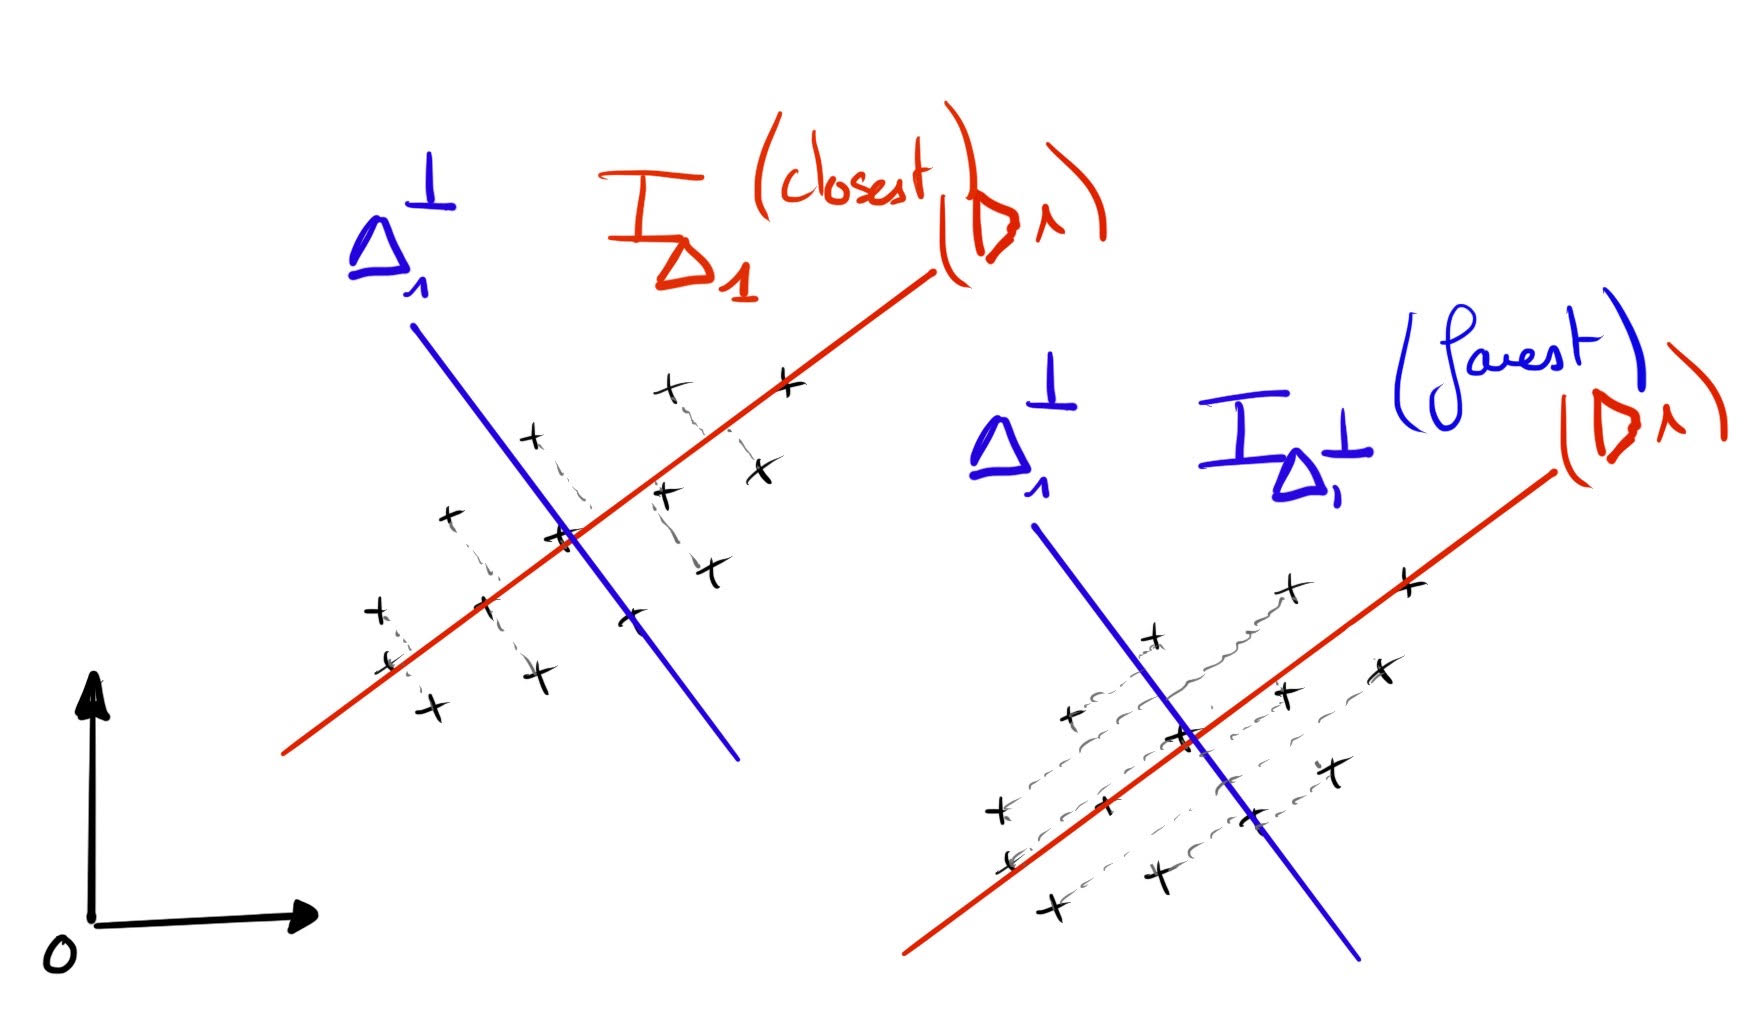
\includegraphics[width=.7\textwidth]{minimum_inertia}
  
\end{frame}

\begin{frame}
  \frametitle{Finding the best axis (3)}

\begin{columns}
  \begin{column}{.5\textwidth}
  \begin{block}{Stating the problem (algebraically)}
    Find $\bu_1; \|\bu_1 \|=1$ that maximizes
    \begin{equation*}
      \begin{aligned}
        I_{\Delta_1^\bot} & = \frac{1}{n}\sum_{i=1}^n \distance(\bx_i,\Delta_1^\bot)^2 \\ 
        & = \frac{1}{n}\sum_{i=1}^n \bu_1^\top (\bx_i - \bar{\bx})(\bx_i - \bar{\bx})^\top \bu_1 \\
        & = \bu_1^\top \left( \sum_{i=1}^n \frac{1}{n}(\bx_i - \bar{\bx})(\bx_i - \bar{\bx})^\top \right)  \bu_1 \\
        & = \bu_1^\top \hat{\bSigma}  \bu_1
      \end{aligned}
    \end{equation*} 
  \end{block}  
  \end{column}
  \begin{column}{.45\textwidth}
  \begin{figure}
    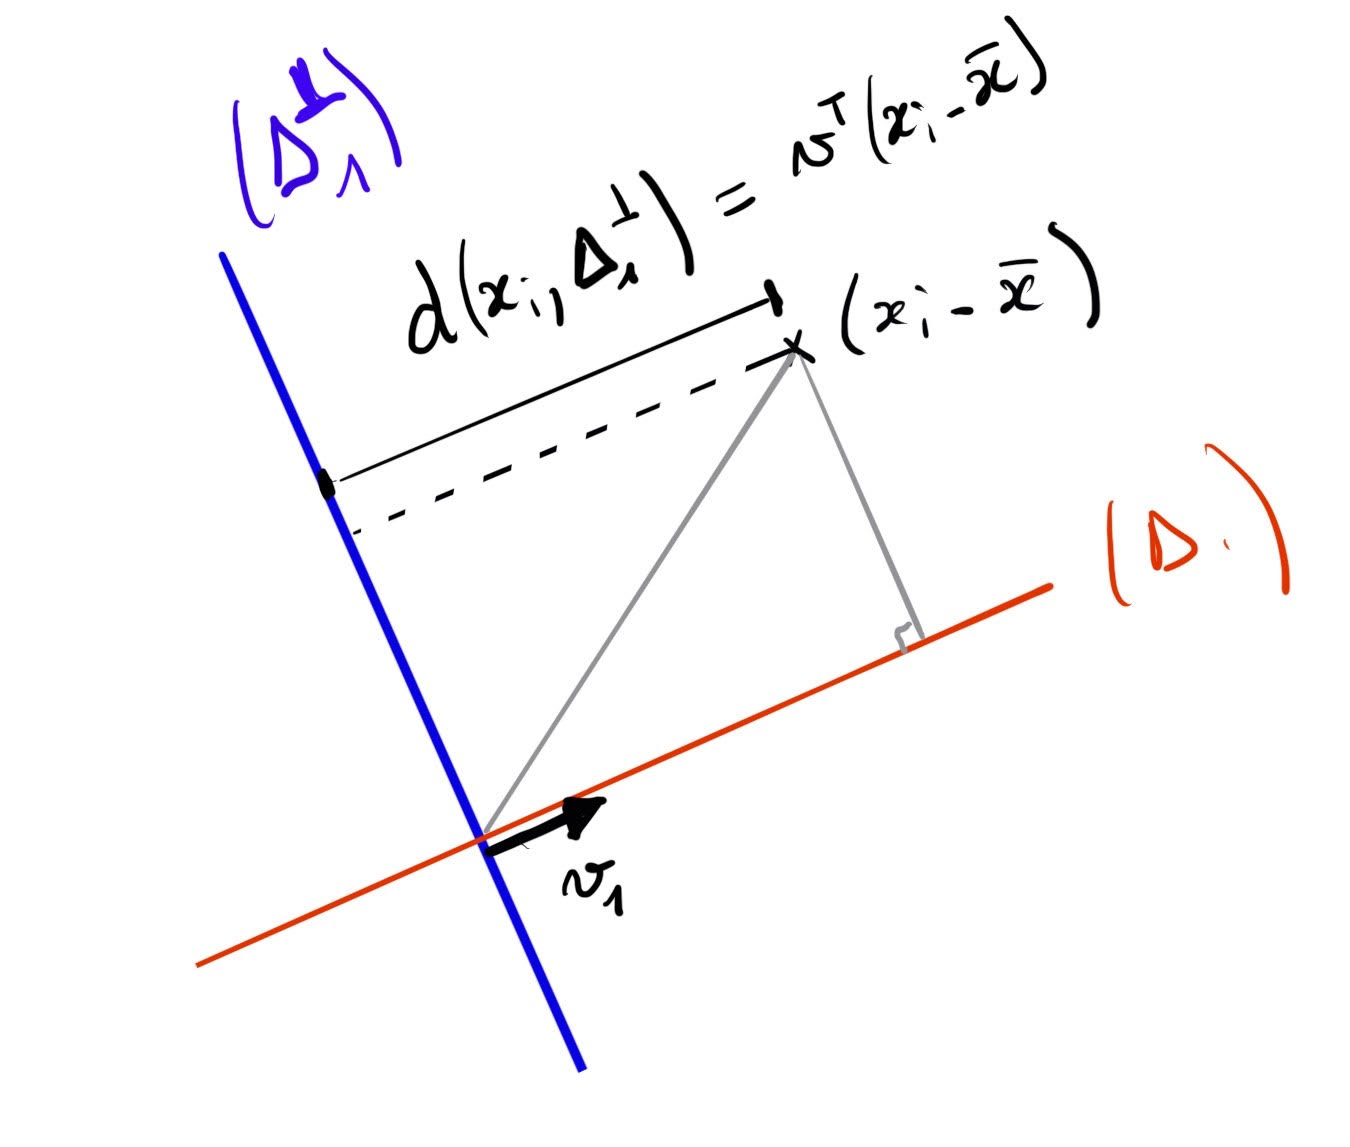
\includegraphics[width=.9\textwidth]{solving_inertia}
    \caption{Geometrical insight}
  \end{figure}
  \end{column}
\end{columns}
  
\end{frame}

\begin{frame}
  \frametitle{Finding the best axis (4)}

  We solve a simple constraint maximization problem with the method of Lagrange multipliers:
  
  \begin{equation*}
    \maximize_{\bu_1: \|\bu_1\| = 1 } \bu_1^\top \hat\bSigma \bu_1 \Leftrightarrow \maximize_{\bu_1\in\Rset^p, \lambda_1 > 0} \bu_1^\top \hat\bSigma \bu_1 - \lambda_1 (\|\bu_1\|^2 - 1)
  \end{equation*}
  
  By straightforward (vector) differentiation, an using that $\bu_1^\top \bu_1 = 1$
  \begin{equation*}
    \left\{\begin{aligned}
      2\hat\bSigma \bu_1 - 2\lambda_1 \bu_1 & = 0 \\  
      \bu_1^\top \bu_1 - 1 & = 0 \\  
    \end{aligned}\right. \Leftrightarrow
    \left\{\begin{aligned}
      \hat\bSigma \bu_1 & = \lambda_1 \bu_1  \\  
      \bu_1^\top \hat\bSigma \bu_1 & = \lambda_1 \bu_1^\top \bu_1 = \lambda_1 = I_{\Delta_1}^\bot \\  
    \end{aligned}\right.
  \end{equation*}
  
  \begin{itemize} 
     \item $\bu_1$ is the first eigen vector of $\hat{\bSigma}$
     \item $\lambda_1$ is the first eigen value of $\hat{\bSigma}$
   \end{itemize} 
  
  $\rightsquigarrow$ \alert{\bf $\Delta_1$ is defined by the first eigen vector of $\hat\bSigma$}\\
  $\rightsquigarrow$ \alert{\bf Variance "carried" by $\Delta_1$ is equal to the largest eigen value of $\hat\bSigma$}
  
\end{frame}

\begin{frame}
  \frametitle{Finding the following axes}

  \begin{block}{Second best axis}
    Find $\Delta_2$ with dimension 1, director vector $\bu_2$ orthogonal to $\Delta_1$ solving
    \begin{equation*}
        \maximize_{\bu_2 \in \Rset^p} I_{\Delta_2^\bot} = \bu_2^\top \hat{\bSigma}\bu_2, \quad \text{with } \|\bu_2\| = 1, \bu_1^\top \bu_2 = 0.
    \end{equation*} 
  $\rightsquigarrow$ $\bu_2$ is the second eigen vector of $\hat\bSigma$ with eigen value $\lambda_2$
  \end{block}
  
  \vfill
  \pause
  
  \begin{block}{And so on!}
    PCA is roughly a matrix factorisation problem 
    \begin{equation*}
      \hat\bSigma = \bU \boldsymbol\Lambda \bU^\top, \quad
      \bU = \begin{pmatrix}
      \bu_1 & \bu_2, & \dots & \bu_p
      \end{pmatrix}, \quad \boldsymbol\Lambda = \diag(\lambda_1, \dots, \lambda_p)
    \end{equation*}
    \hspace{-.5cm}
  \begin{itemize}
    \item $\bU$ is an orthogonal matrix of normalized eigen vectors.
    \item $\boldsymbol\Lambda$ is diagonal matrix of  ordered eigen values.
  \end{itemize}
  \end{block}
\end{frame}

\begin{frame}
  \frametitle{Interpretation in $\Rset^p$}
    
  $\bV$ describes a new orthogonal basis and a rotation of data in this basis\\
  $\rightsquigarrow$ PCA is an appropriate rotation on axes that maximizes the variance

  \begin{equation*}
    \left\{\begin{array}{ccccc}
      \Delta_1 & \oplus & \dots & \oplus & \Delta_p \\
      \bu_1 & \bot & \dots & \bot & \bu_2 \\
      \lambda_1 & > & \dots & > & \lambda_p \\
      I_{\Delta_1^\bot} & > & \dots & > & I_{\Delta_p^\bot} \\
    \end{array}\right.
  \end{equation*}

  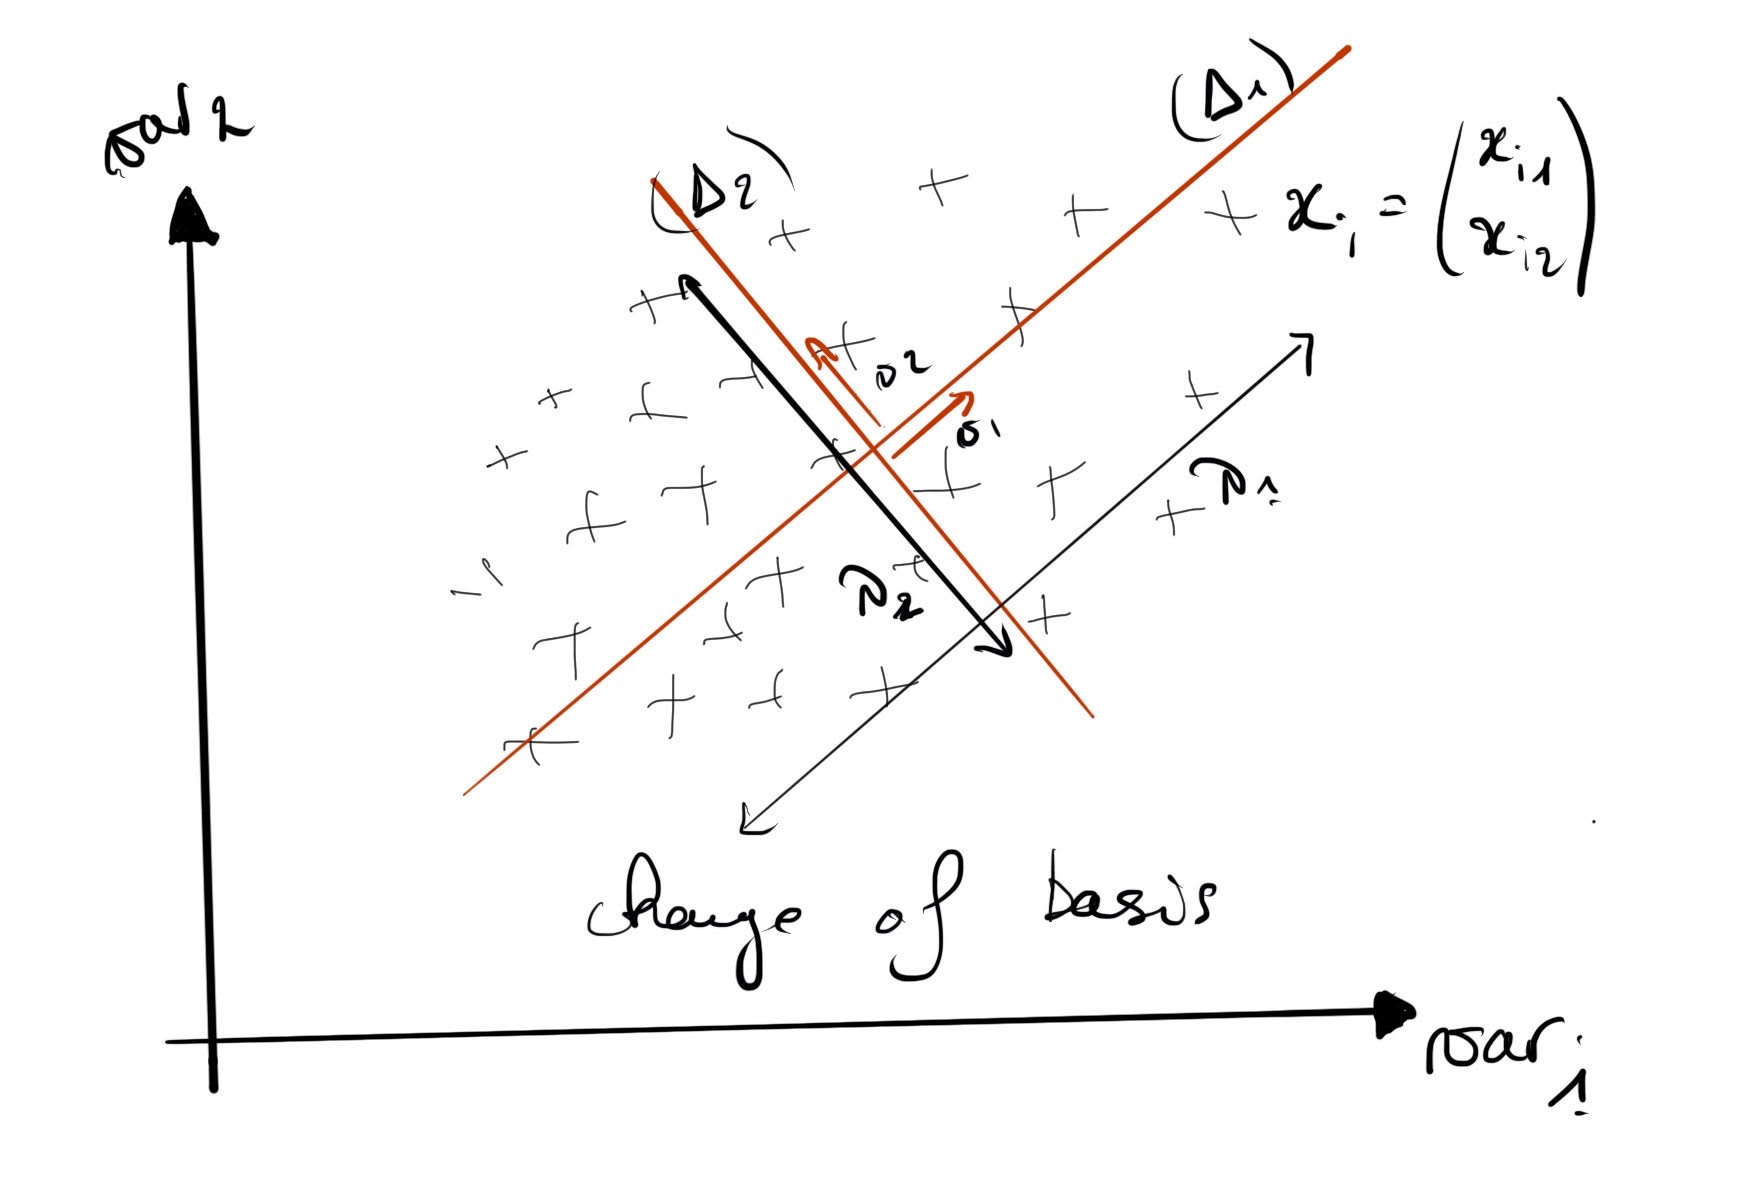
\includegraphics[width=.6\textwidth]{rotation}
\end{frame}
